\section{Implementação do Memora}
\label{sec:implementacao-memora}

\subsection{Tecnologias e organização da aplicação}

O Memora foi implementado com HTML, CSS e JavaScript, a partir do código do Beto, de Leandro Gabriel e colaboradores \cite{gabriel2022beto}. HTML estrutura os elementos da interface, CSS define sua apresentação e JavaScript controla a configuração, a simulação e as interações. A aplicação executa no navegador e é disponibilizada como um site estático, sem exigir instalação pelo estudante. A licença MIT e a atribuição ao código de origem foram preservadas.

A implementação separa a interface da lógica da simulação. A interface recebe os parâmetros, comunica erros, controla a reprodução e apresenta resultados. O núcleo interpreta os endereços, aplica o mapeamento e a política de substituição e produz o estado da cache e as estatísticas. Para cada acesso concluído, são conservadas cópias do estado anterior e do posterior, permitindo consultar o histórico sem alterar a execução.

Foram preservados os três mapeamentos e as políticas FIFO, LRU e aleatória já existentes no Beto. O desenvolvimento concentrou-se em validação, organização dos campos, explicações, visibilidade dos metadados e controle da execução. O Memora\footnote{Disponível em: \url{https://luizjr2001.github.io/memora-cache-simulator-tcc/}.} e seu código-fonte\footnote{Disponível em: \url{https://github.com/LuizJr2001/memora-cache-simulator-tcc}.} estão disponíveis para consulta. O processo foi acompanhado por Kanban e registros de requisitos, decisões e alterações, de modo a relacionar os problemas às mudanças realizadas.

\subsection{Configuração e prevenção de erros}

A etapa Configurar reúne os parâmetros da memória principal e da cache e a sequência de endereços. A validação ocorre durante a edição e é repetida antes de iniciar a simulação. Cada endereço representa uma palavra da memória principal; o rótulo herdado da interface utiliza o termo ``célula'' para essa unidade. Uma memória com 4096 palavras, por exemplo, possui endereços de 0 a 4095. O tamanho em bytes de cada palavra altera a capacidade, mas não a quantidade de endereços nesse modelo.

Os parâmetros de quantidade de palavras, palavras por bloco, linhas e vias devem ser potências de dois compatíveis entre si. Entradas inválidas recebem mensagens próximas dos campos, explicando o que precisa ser corrigido. Os valores não são substituídos silenciosamente. A sequência aceita até 1000 endereços; o gerador de endereços aleatórios utiliza os limites da memória configurada e informa que substituirá a sequência editada. Também é possível carregar um exemplo pronto.

A prévia apresenta os campos do endereço conforme o mapeamento escolhido: \textit{tag}, linha ou conjunto e deslocamento. Ao selecionar Iniciar simulação, os dados são preparados e a etapa Simular é aberta com zero acessos processados, aguardando uma ação de reprodução ou avanço. A Figura~\ref{fig:memora-configurar-atual} apresenta essa organização.

\begin{figure}[!htbp]\centering
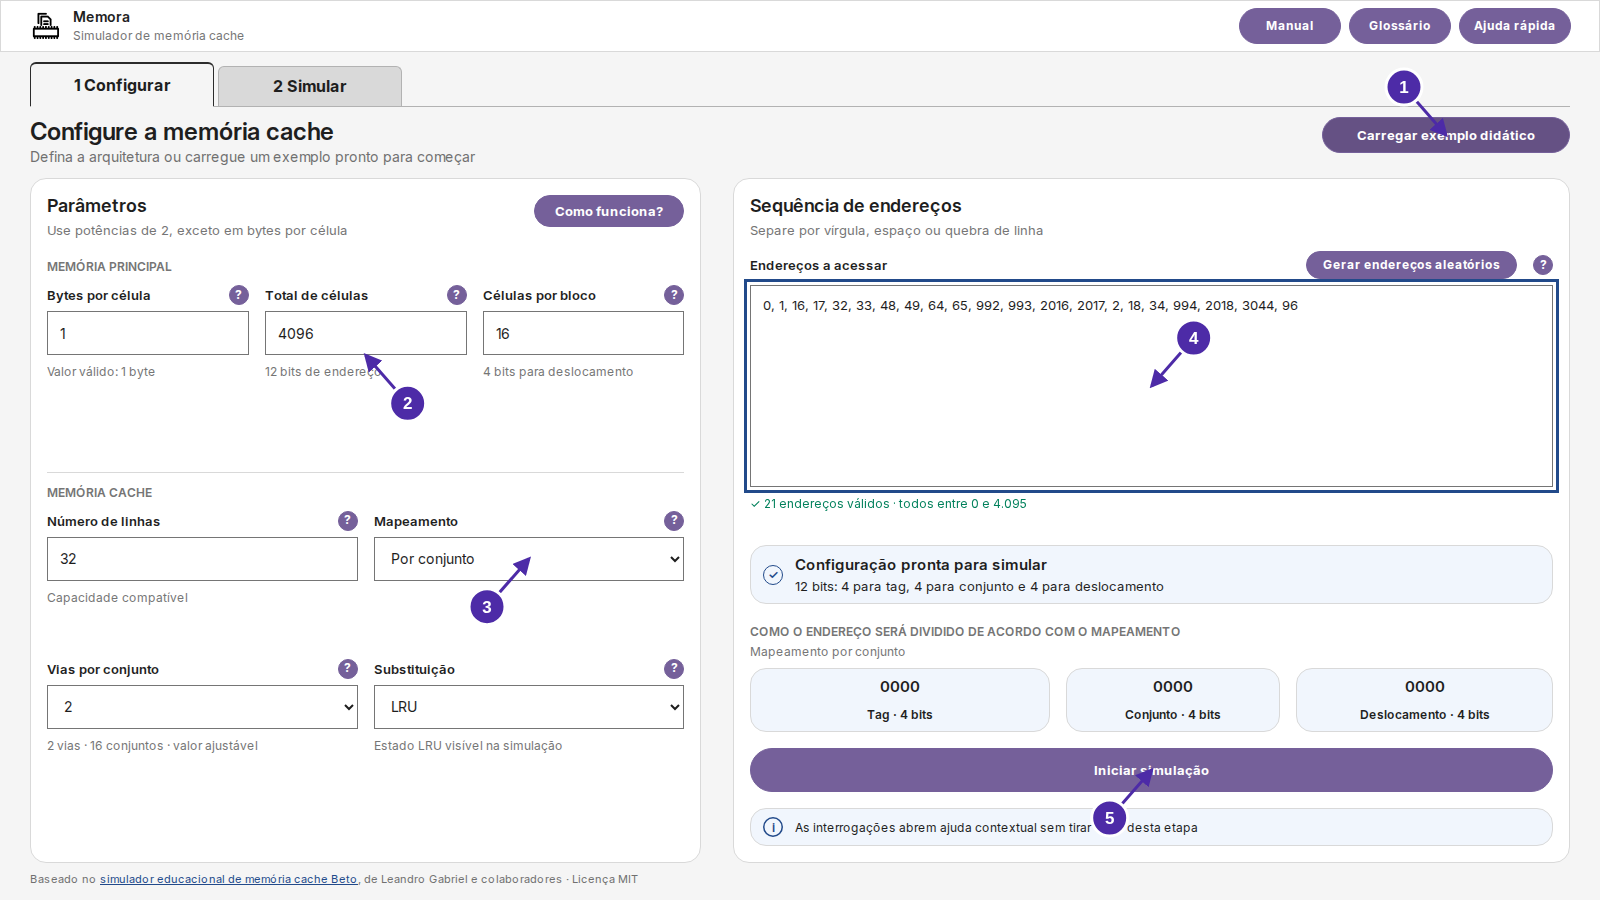
\includegraphics[width=\linewidth,height=.39\textheight,keepaspectratio]{figuras/manual/configurar.png}
\caption{Interface de configuração do Memora.}\label{fig:memora-configurar-atual}
\par\footnotesize Fonte: captura própria da aplicação; cenário ilustrativo.
\end{figure}

\subsection{Execução, histórico e comparação de estados}

A etapa Simular permite executar a sequência automaticamente ou avançar manualmente. Com as etapas detalhadas ativadas, cada acesso percorre decomposição, consulta, determinação do resultado, seleção da via, atualização da cache e conclusão. No modo resumido, cada avanço conclui um acesso. O controle de velocidade ajusta o ritmo de reprodução; o avanço para o final conclui os acessos restantes, e Reiniciar permite recomeçar o cenário.

A cache apresenta validade, \textit{tag}, blocos e palavras, além da recência LRU quando aplicável. A posição 1 indica a via mais recente e não deve ser confundida com o número da via. A indicação de progresso e os totais de acertos e faltas permanecem visíveis durante a execução. Ao final, o progresso recebe indicação de conclusão. A Figura~\ref{fig:memora-simular-atual} mostra os controles e as informações reunidos nessa etapa.

\begin{figure}[!htbp]\centering
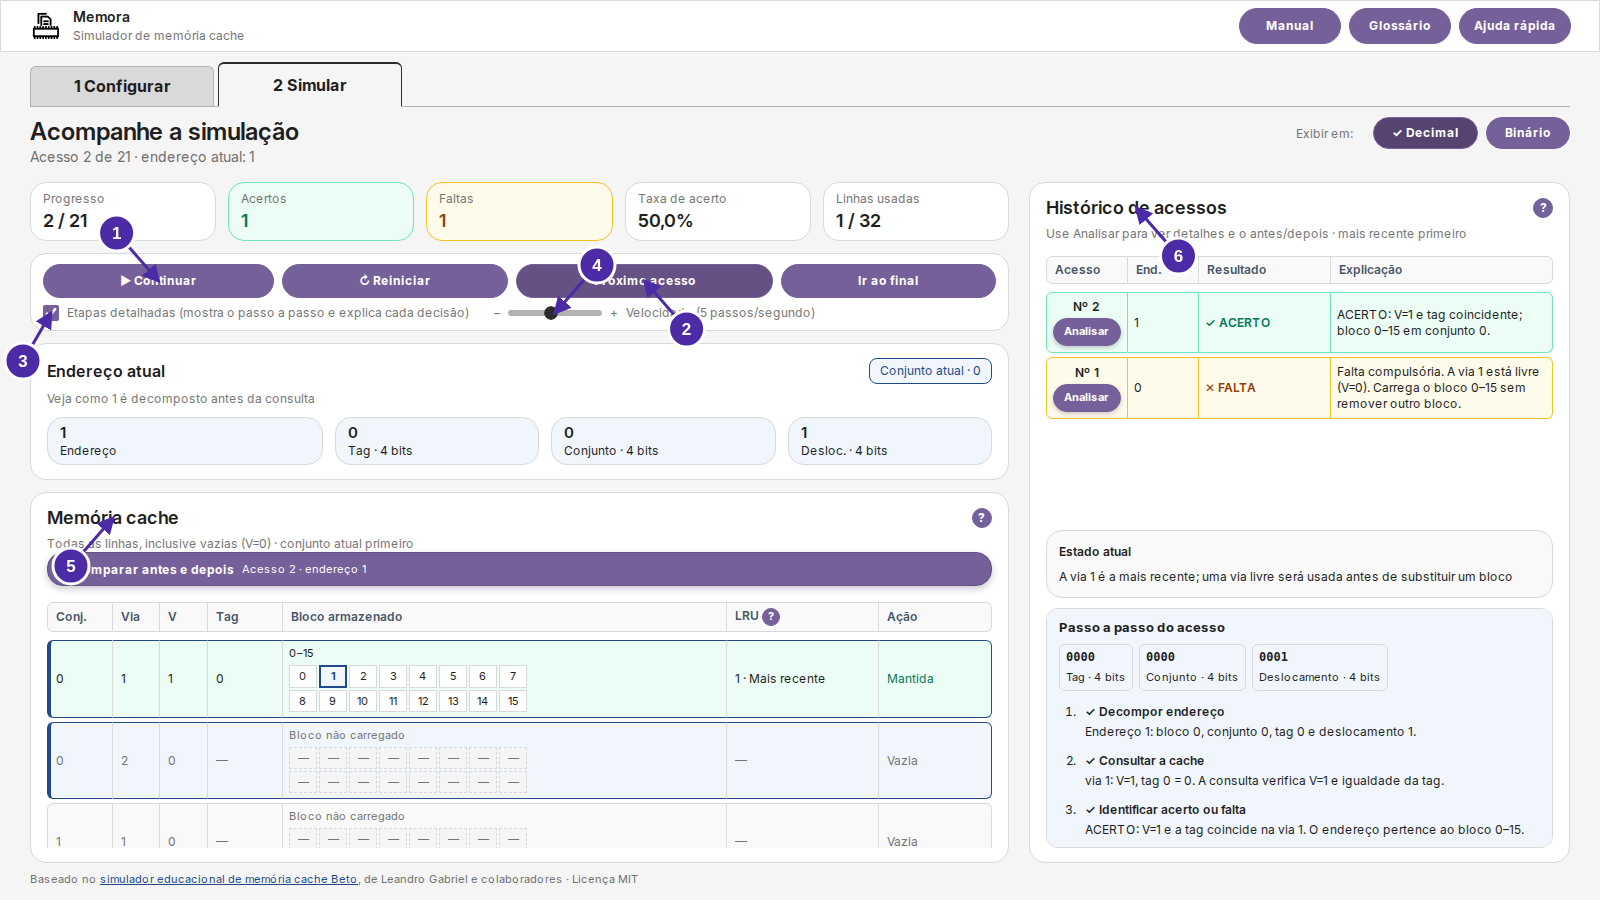
\includegraphics[width=\linewidth,height=.39\textheight,keepaspectratio]{figuras/manual/simular.png}
\caption{Interface de simulação do Memora.}\label{fig:memora-simular-atual}
\par\footnotesize Fonte: captura própria da aplicação; cenário ilustrativo.
\end{figure}

O histórico conserva os acessos concluídos e oferece a ação Analisar junto ao número de cada um. A seleção abre uma comparação do estado da cache antes e depois daquele acesso, destacando os blocos envolvidos e o motivo da substituição. A consulta utiliza os estados registrados, sem recalcular os contadores nem sortear novamente uma vítima na política aleatória. Abrir a comparação pausa a reprodução, e o comando Voltar ao estado atual permite retornar à visualização da execução.

\subsection{Ajuda e identidade visual}

As explicações estão próximas dos elementos a que se referem. O estudante pode consultar o significado de um parâmetro, regras de preenchimento, um exemplo didático, o Glossário e a Ajuda rápida. Os painéis de ajuda podem ser fechados por teclado e devolvem o foco ao controle que os abriu. A opção Decimal/Binário altera a apresentação dos endereços sem modificar os valores simulados.

Os botões utilizam preenchimento roxo e texto branco, enquanto os painéis informativos adotam fundo azul claro. A diferenciação entre campos, ações e informações foi preservada na implementação. O par de cores do botão principal apresenta razão de contraste de 5,39:1, superior a 4,5:1 para texto comum nas WCAG 2.2 \cite{wcagContraste2026}. Esse cálculo se refere ao par de cores examinado, sem representar uma avaliação completa de acessibilidade.

\subsection{Verificação técnica}
\label{sec:verificacao}

A verificação registrada durante o desenvolvimento incluiu 78 testes da lógica e dos controladores no ambiente Node e 94 cenários de interação em Chromium. Foram examinados mapeamentos, substituições, validação, estados históricos, uso por teclado e diferentes dimensões de tela. Os testes da aplicação e a geração do site apoiaram a integração incremental das alterações.

Foram usados cenários com resultados conhecidos para verificar a interpretação dos endereços e a atualização da cache. Um cenário direto com 21 acessos termina em 13 acertos e 8 faltas. Outro, associativo por conjunto com duas vias e LRU, termina em 12 acertos e 9 faltas e permite examinar uma substituição. Seus parâmetros e sequências estão no Apêndice~\ref{ap:roteiro-memora}. A verificação técnica complementa a análise da experiência de uso com estudantes, apresentada a seguir.
